\documentclass[a4paper,11pt]{article}
\usepackage[utf8]{inputenc}
\usepackage[margin=0.8in]{geometry}
\usepackage{tikz}
\usetikzlibrary{arrows.meta}

\begin{document}

\section*{Historical and Structural Analysis: Mestre's Evolution}

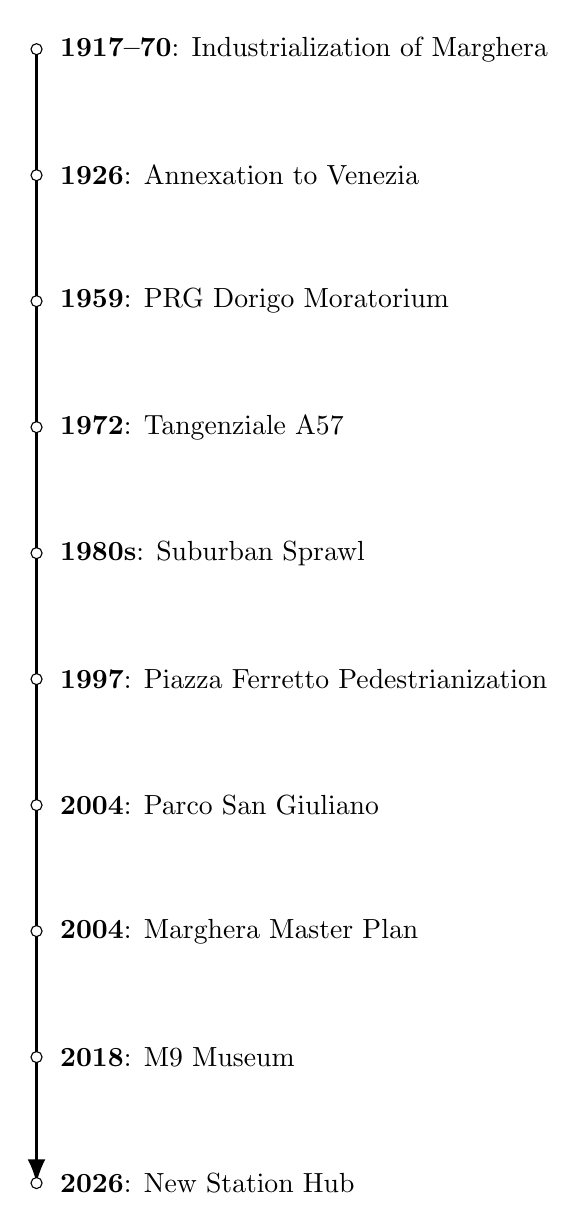
\begin{tikzpicture}[x=1cm, y=0.8cm]
    % Vertical Arrow
    \draw[->, thick, -{Latex[length=3mm]}] (0,0) -- (0,-18);

    % Timeline Nodes
    \foreach \y/\year/\event in {
        0/1917–70/Industrialization of Marghera,
        -2/1926/Annexation to Venezia,
        -4/1959/PRG Dorigo Moratorium,
        -6/1972/Tangenziale A57,
        -8/1980s/Suburban Sprawl,
        -10/1997/Piazza Ferretto Pedestrianization,
        -12/2004/Parco San Giuliano,
        -14/2004/Marghera Master Plan,
        -16/2018/M9 Museum,
        -18/2026/New Station Hub
    } {
        \draw[fill=white] (0,\y) circle (2pt) node[right=5pt] {\textbf{\year}: \event};
    }
\end{tikzpicture}

\newpage

\section*{Evolutionary Analysis and Structural Determinants}

\subsection*{The Founding Moment}
The systemic trajectory originates in the \textbf{1917–1970 Industrialization of Porto Marghera}. This is the causal beginning: it created the demographic mass and the monofunctional economic dependency that today's urban regeneration efforts still struggle to overcome. 

\subsection*{Critical Events \& Lock-in Factors}
\begin{itemize}
    \item \textbf{1926 Annexation (Political Lock-in):} An irreversible administrative choice. By surrendering autonomous civic status, Mestre became a subordinate functional periphery, permanently hindering independent urban identity.
    \item \textbf{1959–61 PRG Dorigo/Moratorium (Legal Irreversibility):} The choice not to impose strict zoning led to chaotic, low-density sprawl. This "freedom of expansion" is now a rigid constraint, leaving the city without a central nervous system.
    \item \textbf{1972 Tangenziale A57 (Infrastructural Irreversibility):} A technological lock-in. This infrastructure cemented the "city of transit" model, creating physical barriers that today discourage the pedestrian walkability required for social hubs.
\end{itemize}

\subsection*{Systemic Trap: The "Flagship" Strategy}
Current decision-makers favor "flagship" projects (M9 Museum, Parco San Giuliano, New Station). These represent a \textbf{Systemic Trap}:
\begin{itemize}
    \item \textbf{Why it's a trap:} Flagships are top-down, predictable, and politically visible. They do not require the structural compromise of density and social mix.
    \item \textbf{The Trade-off:} By prioritizing isolated landmarks, the system maintains its rigidity. True regeneration would require a \textit{diffused network of places}, which demands higher social investment with less immediate political return.
\end{itemize}

\subsection*{Strategic Interventions \& Leverage Points}
Understanding that Mestre is \textit{rigid} rather than \textit{flexible} is key. Strategic intervention must avoid "naive solutions" (e.g., just building another monument). Instead, leverage points should focus on:
\begin{enumerate}
    \item \textbf{Decentralized Density:} Redirecting investment from central flagships to diffused peripheral hubs.
    \item \textbf{Mobility Trade-off:} Reducing the car-dependency established in the 1970s to favor social connectivity.
\end{enumerate}

\end{document}
